\documentclass[crop,tikz]{standalone}
\usepackage{pgf,pgfplots}
\usetikzlibrary{shapes,arrows,positioning}
\begin{document}

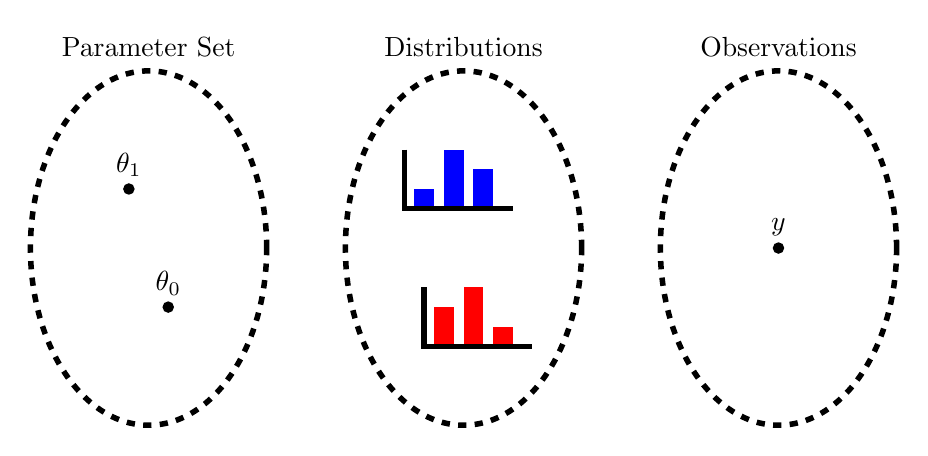
\begin{tikzpicture}
[node distance=2cm, draw=black, line width=2pt,
  myset/.style={ellipse, minimum width=30mm, minimum height=45mm, draw=black, dashed},
  mydot/.style={circle, minimum size=0.5pt, draw=black, fill=black}
]
  \node[myset] (parameters) at (0,0) [label=Parameter Set]{};
  \node[myset] (distributions) at (4,0) [label=Distributions]{};
  \node[myset] (observations) at (8,0) [label=Observations]{};

  \draw[fill=black] (0.25,-0.75) circle (1pt) node[above] {$\theta_0$};
  \draw[fill=black] (-0.25,0.75) circle (1pt) node[above] {$\theta_1$};

  \draw[draw=none,fill=blue] (3.375,0.5) rectangle (3.625,0.75);
  \draw[draw=none,fill=blue] (3.75,0.5) rectangle (4,1.25);
  \draw[draw=none,fill=blue] (4.125,0.5) rectangle (4.375,1);
  \draw (3.25,1.25) -- (3.25,0.5) -- (4.625, 0.5);

  \draw[draw=none,fill=red] (3.625,-1.25) rectangle (3.875,-0.75);
  \draw[draw=none,fill=red] (4,-1.25) rectangle (4.25,-0.5);
  \draw[draw=none,fill=red] (4.375,-1.25) rectangle (4.625,-1);
  \draw (3.5,-0.5) -- (3.5,-1.25) -- (4.875, -1.25);

  \draw[fill=black] (8,0) circle (1pt) node[above] {$y$};
\end{tikzpicture}
\end{document}
